\documentclass{article}

\title{Lab-4}
\author{2347139}
\date{\today}


\usepackage{listings}
\usepackage{color}
\usepackage{graphicx}

\definecolor{dkgreen}{rgb}{0,0.6,0}
\definecolor{gray}{rgb}{0.5,0.5,0.5}
\definecolor{mauve}{rgb}{0.58,0,0.82}

\lstset{frame=tb,
  language=Java,
  aboveskip=3mm,
  belowskip=3mm,
  showstringspaces=false,
  columns=flexible,
  basicstyle={\small\ttfamily},
  numbers=left,
  numberstyle=\tiny\color{gray},
  keywordstyle=\color{blue},
  commentstyle=\color{dkgreen},
  stringstyle=\color{mauve},
  breaklines=true,
  breakatwhitespace=true,
  tabsize=3
}
\begin{document}
\maketitle
\begin{lstlisting}
    interface Guild {
    public void createGuild(String guildName);

    public void getBotPermission(int permission);
}

interface Bot extends Guild {
    public void getMembers();

    public void slashCommand(String user);
}

class DiscordBot implements Bot {
    public void createGuild(String guildName) {
        System.out.println("Created a guild " + guildName + " associated to the bot");
    }

    public void getBotPermission(int permission) {
        boolean isAdmin = true;
        boolean isMod = true;
        boolean BAN_MEMBERS = true;
        boolean KICK_MEMBERS = true;
        if (permission == 0) {
            System.out.println("The Bot created has 0 permission");
        }
        if (isAdmin && isMod && BAN_MEMBERS && KICK_MEMBERS) {
            System.out.println("The Bot is set full permission");
        }

    }

    public void getMembers() {
        System.out.println("Getting members of the text channel");
        System.out.println("Channel members are : Elumeveguy\n" + //
                "Emojorekes\n" + //
                "Eroxihisom\n" + //
                "Ulelabutuk\n" + //
                "Ayibiciqeb\n" + //
                "Oguyocuxas\n" + //
                "Uxibabujen\n" + //
                "Epiwimaguk\n" + //
                "Idenefibiy\n" + //
                "Amarebamat");

    }

    public void slashCommand(String user) {
        // String command='ban';
        System.out.println("Ban User ");
        System.out.println("user " + user + " is banned");

    }

    public String name;
    public String discordServer;

    DiscordBot(String name, String discordServer) {
        this.name = name;
        this.discordServer = discordServer;
    }

    public void getBotDetails() {
        System.out.println("your account name is " + name);
        System.out.println("your Discord server name is " + discordServer);

    }

}

class Discord {
    public static void main(String args[]) {
        DiscordBot bot = new DiscordBot("bob_account", "bobServer");
        bot.createGuild("Capture_the_flag_bot");
        bot.getBotPermission(122);
        bot.getMembers();
        bot.slashCommand("bob");
        bot.getBotDetails();
    }
}
\end{lstlisting}

\section*{Output}
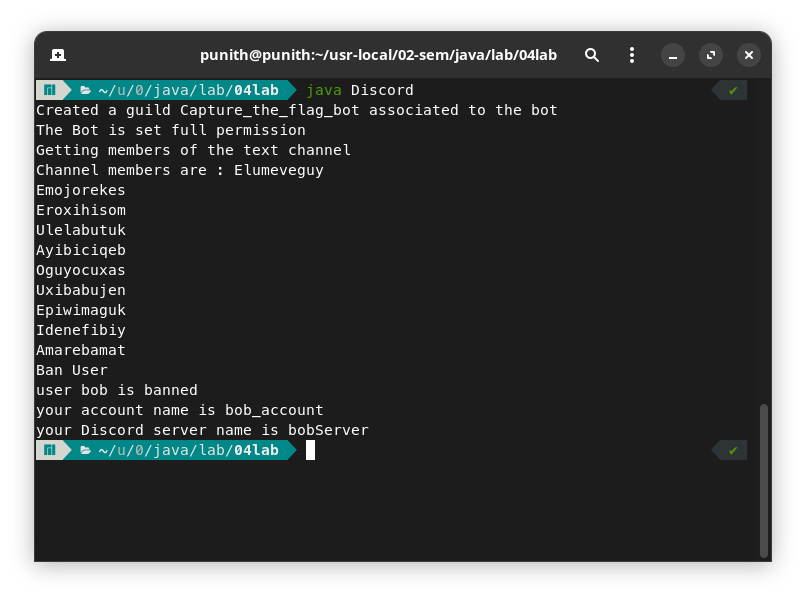
\includegraphics[width=11cm, height=9cm]{./images/01.png}

\end{document}
